\section{Evaluation}

In this section we present an evaluation of our approach. Our evaluation comprises two parts: (i) a usability evaluation involving two experiments with two groups of students (Section~\ref{sec:usab}); and (ii) a preliminary analysis of the performance overhead of our approach (Section~\ref{sec:perf}).  The exact input, instructions, and any additional document we have used in this section are available at \cite{repo}.

\subsection{Usability Evaluation}\label{sec:usab}

We ran empirical evaluation to measure the efficiency of deadlock exceptions with regard to problem solving speed and accuracy. We defined two research questions for this evaluation: {\bf RQ1.} Is the time spent to identify the bug reduced using our implementation? {\bf RQ2.} Is the accuracy in the identification of the causes of a deadlock bug improved for developers using our approach? For the second question, each answer was evaluated based on three criteria with three possible values each: 0 for absence, 0.5 for partially present and 1 for fully present. First criteria, \emph{A}, stands for "correctly classified problem as deadlock"; second criteria, \emph{B}, means "classified problem as different from deadlock"; and lastly, \emph{C} means "correctly identified method calls involved in the deadlock". Whenever $(A - B) + C \geq 1.5$ is true, we defined it as a correct answer (that is, whenever the bug was described as deadlock and at least one of the methods involved in the deadlock were identified correctly).

We wrote two programs with different levels of complexity which were presented in the same order for all subjects. The first program, known as \emph{Bank}, contained 4 classes spread among 4 files, 3 threads, 3 explicit locks, and a mean of 82 lines of code per file. The second program, known as \emph{Eclipse}, had 15 classes spread in 11 files, 4 threads, 5 explicit locks, and a mean of 40 lines of code per file. Each program could use either \emph{LockA} or \emph{LockB}, where \emph{LockA} was our implementation with deadlock detection on at least one thread involved in a deadlock, while \emph{LockB} was just the default \emph{ReentrantLock} implementation. Each student was assigned to either group A or B randomly. In group A, students would start with \emph{LockA} in the first program but use \emph{LockB} on the second program; meanwhile, in group B students would have the locks in opposite order.

The two experiments had similar setups but differed in terms of the subjects. For the first experiment, the subjects comprised a group of third-year undergraduate students who underwent an 18-hour concurrent programming course. The course included a number of programming assignments. The experiment was conducted as a test for the course. The subjects of the second experiment were  graduate students enrolled in master's degree or PhD program attending a 40-hour Parallel Programming course with a focus on algorithms and data structures. They had classes about advanced concepts of parallel programming and had practical exercises, including implementing a number of different locking approaches. The participants in the second experiment were all volunteers and were not required to take part in it. Also, for both experiments, the assignments were the same. It asked students to identify any problems they could with the provided programs. All students started the experiment with program \emph{Bank}. When they finished, they received the second program, \emph{Eclipse}. When a student finished one of the programs, we set a timestamp on it. The timestamp was written based on a chronometer visible to everyone in the laboratory. For the first group (undergraduate students), we allowed 90 minutes per program. For the second group (graduate students), we allowed 60 minutes per program. 

\subsubsection{Time Analysis.}

We defined the following hypothesis to answer {\bf RQ1}:

\begin{equation}
  H_{0} : \mu_{TimeLockA} \geq \mu_{TimeLockB}
\end{equation}
\begin{equation}
  H_{1} : \mu_{TimeLockA} < \mu_{TimeLockB}
\end{equation}

We used Latin Square Design~\cite{box} to control two factors that might affect the metrics: subjects and program complexity.
Programs \emph{Bank} and \emph{Eclipse} had complexity easy and difficult respectively, while \emph{LockA} and \emph{LockB} were the two possible treatments we wanted to compare.
Since we had N subjects, 2 programs and 2 possible treatments, we disposed subjects in rows and programs in columns of latin squares, randomly assigning in each cell of the square a treatment that could be \emph{LockA} or \emph{LockB}, but also guaranteeing that for any given row or column in this square, each treatment appeared only once. Consequently, we have replication, local control and randomization which are the three principles of experiment design \cite{box}. Time analysis was conducted with R Statistical Software using the inputs extracted from each day. We used the linear model described in Figure~\ref{fig:model} that considers the effect of different factors on the response variable as proposed by other authors~\cite{paola}, including the effect between each replica and treatment~\cite{sanchez}.

\begin{figure}
\begin{center}
$Y_{lijk} = \mu + \tau_{l} + \tau\alpha_{li} + \beta_{j} + \gamma_{k} + \tau\gamma_{lk} + \epsilon_{lijk}$\\
\vspace{4mm}
\begin{tabular}{ll}
$Y_{lijk}$ & - response of $l_{th}$ replica, $i_{th}$ student, $j_{th}$ program, $k_{th}$ lock \\
$\tau_{l}$ & - effect of $l_{th}$ replica \\
$\tau\alpha_{li}$ & - effect of interaction between $l_{th}$ replica and $i_{th}$ student \\
$\beta_{j}$ & - effect of $j_{th}$ program \\
$\gamma_{k}$ & - effect of $k_{th}$ lock \\
$\tau\gamma_{lk}$ & - effect of interaction between $l_{th}$ replica and $k_{th}$ lock \\
$\epsilon_{lijk}$ & - random error \\
\end{tabular}
\caption{Regression model.}\label{fig:model}
\end{center}
\end{figure}

Initially, we plotted box-plot graphics shown in Figure~\ref{fig:boxplots} for both experiments and calculated the means for time spent in Table~\ref{tab:mean1} and Table~\ref{tab:mean2}, where we can observe that students finished the exercise faster on the average when using our approach: 16.87\% less time on the first group and 30.70\% less on the second group. Then we ran Box-Cox transformation to reduce anomalies such as non-additivity and non-normality. The value of $\lambda$ at the maximum point in the curve drawn by box-cox function in R was not approximately 1 ($\lambda = 5$), thus we should apply the transformation: on our regression model, $Y_{lijk}$ should be powered to $\lambda$. We did the same on the second experiment as $\lambda = 1.3636$.

\begin{figure}%
    \centering
    \subfloat[First experiment]{{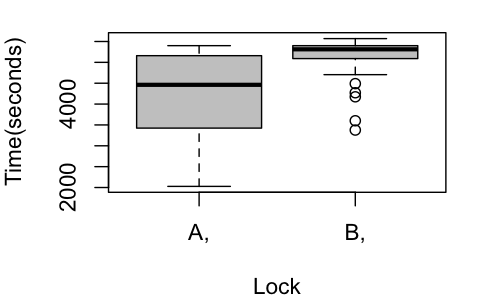
\includegraphics[width=5cm,natwidth=475,natheight=343]{img/u1.png} }}%
    \qquad
    \subfloat[Second experiment]{{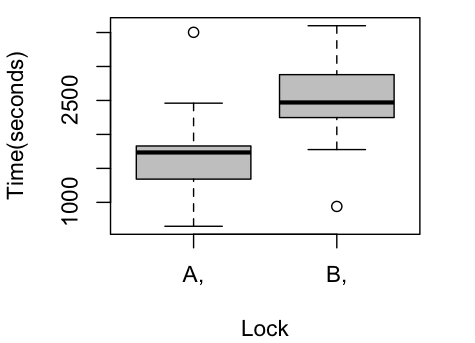
\includegraphics[width=5cm,natwidth=488,natheight=303]{img/g1.png} }}%
    \caption{Box-plot on both experiment days}\label{fig:boxplots}%
\end{figure}

\begin{table}
\parbox{.45\linewidth}{
\centering
\begin{tabular}{|l|l|l|}
\hline
 & Time Spent (mean)\\
\hline
LockA & 4227.800 seconds \\
LockB & 5086.367 seconds \\
\hline
\end{tabular}
\caption{First group's time spent}\label{tab:mean1}
}
\hfill
\parbox{.45\linewidth}{
\centering
\begin{tabular}{|l|l|l|}
\hline
 & Time Spent (mean)\\
\hline
LockA & 1737.714 seconds \\
LockB & 2507.714 seconds \\
\hline
\end{tabular}
\caption{Second group's time spent}\label{tab:mean2}
}
\end{table}

After applying Box-Cox transformation, we ran Tukey Test of Additivity that checks whether effect model is additive. If the model was additive, then rows and columns of each latin square wouldn't affect significantly the response \cite{box}. Now consider the hypothesis where the null hypothesis ($H_{0}$) says the model is additive and alternative hypothesis ($H_{1}$) says the opposite. In the first experiment, model was additive as we obtained p-value of 0.514 which is not lower than 0.05 and we couldn't reject $H_{0}$; similarly for the second experiment, the model was also additive as p-value found was 0.914.

Finally, we ran the ANOVA (ANalysis Of VAriance) test which compares the effect of treatments on the response variable, providing an approximated p-value for every associated factor. When a variable has \emph{p-value} $< 0.05$, it means that factor was significant to the response. Table~\ref{tab:unova1} and Table~\ref{tab:unova2} shows \textbf{the most important factor as the type of \emph{Lock} for both experiments}, allowing us to reject our null hypothesis defined for {\bf RQ1}. Thus, considering this result and the box plots in Figure~\ref{fig:boxplots}, we can say that the use of our locks promoted faster identification of deadlocks.

\begin{table}%
\begin{center}
\caption{First experiment ANOVA results.}\label{tab:unova1}
\begin{tabular}{|l|l|l|l|l|ll|}
\hline
                & Df &    Sum Sq  &  Mean Sq   & F value & \emph{p-value} &     \\  
Replica         & 14 & 3.8633e+37 & 2.7595e+36 & 1.6553  & 0.1784197 &     \\   
Program         & 1  & 4.1460e+36 & 4.1460e+36 & 2.4869  & 0.1371197 &     \\   
Lock            & 1  & 3.9489e+37 & 3.9489e+37 & 23.6873 & 0.0002492 & *** \\
Replica:Student & 15 & 4.1013e+37 & 2.7342e+36 & 1.6401  & 0.1808595 &     \\  
Replica:Lock    & 14 & 2.4033e+37 & 1.7166e+36 & 1.0297  & 0.4785520 &     \\  
Residuals       & 14 & 2.3340e+37 & 1.6671e+36 &         &           &     \\
\hline
\end{tabular}
\end{center}
\end{table}

\begin{table}%
\begin{center}
\caption{Second experiment ANOVA results.}\label{tab:unova2}
\begin{tabular}{|l|l|l|l|l|ll|}
\hline
                 & Df &    Sum Sq &   Mean Sq  & F value &   Pr(>F) & \\   
\hline
replica          & 6 & 2576883250 &  429480542 & 14.1891 & 0.0025793 & **  \\
program          & 1 &    6875586 &    6875586 &  0.2272 & 0.6505035 &     \\
lock             & 1 & 1958179433 & 1958179433 & 64.6938 & 0.0001975 & *** \\
replica:student  & 7 & 2328154077 &  332593440 & 10.9881 & 0.0047601 & **  \\
replica:lock     & 6 &  823830276 &  137305046 &  4.5362 & 0.0441188 & *   \\
Residuals        & 6 &  181610625 &   30268438 &         &           &     \\
\hline
\end{tabular}
\end{center}
\end{table}

\subsubsection{Accuracy Analysis.}

We used the number of correct answers using each lock to measure accuracy, so we defined the following hypothesis to answer {\bf RQ2}. 

\begin{equation}
  H_{0} : \mu_{CorrectAnswersLockA} \leq \mu_{CorrectAnswersLockB}
\end{equation}
\begin{equation}
  H_{1} : \mu_{CorrectAnswersLockA} > \mu_{CorrectAnswersLockB}
\end{equation}

\begin{table}
\parbox{.45\linewidth}{
\centering
\begin{tabular}{|l|l|l|}
\hline
 & Correct & Incorrect\\
\hline
LockA & 29 & 2\\
LockB & 16 & 15\\
\hline
\end{tabular}
\caption{First group's accuracy}\label{tab:accuracy1}
}
\hfill
\parbox{.45\linewidth}{
\centering
\begin{tabular}{|l|l|l|}
\hline
 & Correct & Incorrect\\
\hline
LockA & 13 & 1\\
LockB & 10 & 4\\
\hline
\end{tabular}
\caption{Second group's accuracy}\label{tab:accuracy2}
}
\end{table}

To compare the accuracy of the subjects using Java's regular {\tt ReentrantLock} and our modified implementation, we employed Fisher's exact test \cite{agresti}. We could not use ANOVA because the data for accuracy is categorical (Correct vs. Incorrect) instead of numerical. 
Applying Fisher's exact test on data from Table~\ref{tab:accuracy1} and Table~\ref{tab:accuracy2}, we can see that undergraduate students results presented a two-tailed P value equals 0.0004: the association between rows (groups) and columns (outcomes) was considered to be extremely statistically significant; consequently, it suggests that an improvement on accuracy occurred due to the use of the proposed approach, where it had 81.25\% more correct answers. However graduate students results only had 30\% more correct answers with a two-tailed P value equals 0.3259, which does not represent statistically significant evidence.

Although we cannot draw strong conclusions regarding improved accuracy, we found some interesting behavior. Some students in the second group were greatly experienced on concurrent programming and they knew how to efficiently find a deadlock using the tools available in their IDE of choice, thus being able to finish the tasks really quickly for both problems. This observation allows us to hypothetize that deadlock exceptions are more helpful for less experienced programmers, but we leave investigation of this matter for future work.

\subsubsection{Threats to Validity}

We must consider a few remarks regarding the validity of our results. First remark: we could have used automated process to handle timestamps rather than manually writing their name with it on the whiteboard once they finished a question to keep track of time limit per subject later; this could potentially reduce overhead and increase timestamp precision.
Secondly, the first group did this experiment in replacement of their actual exam might have impacted the time we measured. We noticed some students spent more time on each question by purpose. We believe that they were reluctant to ask for the next question because they still had plenty of time left and they wanted to make sure it was correct. We did not notice such behavior with the second group of students and we believe it is because they did not have the same pressure to deliver correct results as the first group had.
Third remark is related to programs' complexity: the ones we used to evaluate the students are considerably easier to understand than most programs in real world, but unfortunately we could not use any real world scenario as students would not be able to finish each assignment in time; with that in mind, we created two questions based on real world bugs we found on our bug report studies.

Last remark is about whether we are able to draw conclusions based on students data: some studies suggest that using students as subjects is as good as using industry professionals \cite{staron}; Runes ran an experiment which shows that there's not much significant differences between undergraduate, graduate and industry professionals, with the exception that undergraduate students often take more time to complete the tasks \cite{runes}.

\subsection{Performance Overhead}\label{sec:perf}

We conducted a preliminary set of experiments to analyze the overhead of our approach. We compared our deadlock-safe implementation with the original {\tt ReentrantLock} implementation available in the JDK and with Eclipse's deadlock-safe {\tt OrderedLock} \cite{orderedlock}. {\tt OrderedLock} is similar our approach in the sense that it attempts to detect deadlocks at runtime. However, it aims to be general, detecting $N$-thread deadlocks without much concern for performance. 
OrderedLock deeply relies on Eclipse's code architecture. So, in order to use it in our evaluation, we had to perform some small code changes, removing only Eclipse-specific bits that did not affect the core functionality of {\tt OrderedLock}. The source code for these lock implementations is available elsewhere\cite{repo}.

We developed a synthetic benchmark that creates \emph{N} threads that perform additions to ten integer counters where each increment in a counter is protected by explicit locks. Each thread would have to increment its corresponding counter 1000 times before finishing its execution and the counters were evenly distributed across the threads. Therefore, each counter will have exactly \emph{(N / 10)} threads doing increments on it and higher values of \emph{N} result in higher contention, that is, more threads will compete against each other for a particular counter. In this preliminary evaluation, we have conducted measurements for values of $N$ equal to 10, 50, 100, and 200. Since each thread in the benchmark never acquires more than one lock at the same time, deadlocks cannot occur. We emphasize that this setup is very conservative, since every operation that each thread performs requires locking. Thus, the obtained overhead will be a worst-case estimate and thus much higher than one would encounter in a real-world application~\cite{lozi}. The measurements were made on an Intel CoreTM i7 3632QM Processor (6Mb Cache, 2.2GHz) running Ubuntu 12.04.4 LTS and each cell in Table~\ref{tab:overhead} is the average of 50 executions (preceded by 20 executions that served as a warm-up). 

\begin{table}
\begin{center}
\caption{Benchmark time measurements (in seconds)}\label{tab:overhead}
\begin{tabular}{|l|l|l|l|}
\hline
\# Threads & ReentrantLock & ReentrantLock Modified & OrderedLock \\
\hline
10 & 0.084184 & 0.105729 & 0.159503\\
50 & 0.089094 & 0.136507 & 1.094718\\
100 & 0.090978 & 0.159541 & 3.395974\\
200 & 0.131739 & 0.194075 & 11.258714\\
\hline
\end{tabular}
\end{center}
\end{table}

The difference of results between our implementation and the original ReentrantLock gives a range of increased time from about 50\% to 90\%. Meanwhile, OrderedLock performed a lot worse, reaching a 8446.3\% increase in time for the worst case. To get a rough estimate of the impact that this overhead would have on actual application execution time, we analyzed the results obtained by Lozi et al.~\cite{lozi}. The authors profiled 19 real-world applications and small benchmarks in order to measure the time these systems spend on their critical sections. Worst-case results ranged between 0.3\% and 92.7\%. If we consider the average time spent on the critical sections of 12 of these systems, the impact of our approach on the overall execution time would be \textbf{less than 6\% in the worst case}. The remaining cases are extreme, in the sense that these systems spend more time in their critical sections than out of them~\cite{lozi}. 

